% 	Name		:: 	sthlm Beamer Theme  HEAVILY based on the hsrmbeamer theme (Benjamin Weiss)
%	Author		:: 	Mark Hendry Olson (mark@hendryolson.com)
%	Created		::	2013-07-31
%	Updated		::	June 18, 2015 at 08:45
%	Version		:: 	1.0.2
%	Email		:: 	hendryolson@gmail.com
%	Website		:: 	http://v42.com
%
% 	License		:: 	This file may be distributed and/or modified under the
%                  	GNU Public License.
%
%	Description	::	This presentation is a demonstration of the sthlm beamer
%					theme, which is HEAVILY based on the HSRM beamer theme created by Benjamin Weiss
%					(benjamin.weiss@student.hs-rm.de), which can be found on GitHub
%					<https://github.com/hsrmbeamertheme/hsrmbeamertheme>.


%-=-=-=-=-=-=-=-=-=-=-=-=-=-=-=-=-=-=-=-=-=-=-=-=
%
%        LOADING DOCUMENT
%
%-=-=-=-=-=-=-=-=-=-=-=-=-=-=-=-=-=-=-=-=-=-=-=-=

\documentclass[newPxFont]{beamer}
\usetheme{sthlm}
%\usecolortheme{sthlmv42}

%-=-=-=-=-=-=-=-=-=-=-=-=-=-=-=-=-=-=-=-=-=-=-=-=
%        LOADING PACKAGES
%-=-=-=-=-=-=-=-=-=-=-=-=-=-=-=-=-=-=-=-=-=-=-=-=
\usepackage[utf8]{inputenc}
\usepackage[T1]{fontenc}

%\usepackage{chronology}
\usepackage{chronosys}
\usepackage{subfigure}

%\renewcommand{\event}[3][e]{%
%  \pgfmathsetlength\xstop{(#2-\theyearstart)*\unit}%
%  \ifx #1e%
%    \draw[fill=black,draw=none,opacity=0.5]%
%      (\xstop, 0) circle (.2\unit)%
%      node[opacity=1,rotate=45,right=.2\unit] {#3};%
%  \else%
%    \pgfmathsetlength\xstart{(#1-\theyearstart)*\unit}%
%    \draw[fill=black,draw=none,opacity=0.5,rounded corners=.1\unit]%
%      (\xstart,-.1\unit) rectangle%
%      node[opacity=1,rotate=45,right=.2\unit] {#3} (\xstop,.1\unit);%
%  \fi}%

%-=-=-=-=-=-=-=-=-=-=-=-=-=-=-=-=-=-=-=-=-=-=-=-=
%        BEAMER OPTIONS
%-=-=-=-=-=-=-=-=-=-=-=-=-=-=-=-=-=-=-=-=-=-=-=-=

%\setbeameroption{show notes}

%-=-=-=-=-=-=-=-=-=-=-=-=-=-=-=-=-=-=-=-=-=-=-=-=
%
%	PRESENTATION INFORMATION
%
%-=-=-=-=-=-=-=-=-=-=-=-=-=-=-=-=-=-=-=-=-=-=-=-=

\title{L'entraide un facteur d'irrigation}
\subtitle{Gestion de l'eau dans les pyrenees orientales}
%\date{\small{\jobname}}
%\date{\today}
\date{15 juin 2016}
\author{\texttt{M. Chevallier}, \texttt{E. Delay}, \texttt{J. Linton}}
\institute{\small{Chaire "Capital environnemental et gestion durable des cours d'eau"}\\
\textsc{Geolab}, Université de Limoges.}

\hypersetup{
pdfauthor = {M. Chevallier, E. DELAY, J. Linton},
pdfsubject = {Réclusienne 2016},
pdfkeywords = {water},
pdfmoddate= {D:\pdfdate},
pdfcreator = {}
}

\begin{document}

%-=-=-=-=-=-=-=-=-=-=-=-=-=-=-=-=-=-=-=-=-=-=-=-=
%
%	TITLE PAGE
%
%-=-=-=-=-=-=-=-=-=-=-=-=-=-=-=-=-=-=-=-=-=-=-=-=

\maketitle

%\begin{frame}[plain]
%	\titlepage
%\end{frame}

%-=-=-=-=-=-=-=-=-=-=-=-=-=-=-=-=-=-=-=-=-=-=-=-=
%
%	TABLE OF CONTENTS: OVERVIEW
%
%-=-=-=-=-=-=-=-=-=-=-=-=-=-=-=-=-=-=-=-=-=-=-=-=
%\section*{Overview}
%\begin{frame}{Overview}
%% For longer presentations use hideallsubsections option
%\tableofcontents[hideallsubsections]
%\end{frame}

\section{Contexte semantique}

%-=-=-=-=-=-=-=-=-=-=-=-=-=-=-=-=-=-=-=-=-=-=-=-=
%	FRAME:
%-=-=-=-=-=-=-=-=-=-=-=-=-=-=-=-=-=-=-=-=-=-=-=-=

\begin{frame}[c]{Usage des mots : anglais}
\vspace{-2em}
\begin{figure}
	\centering
	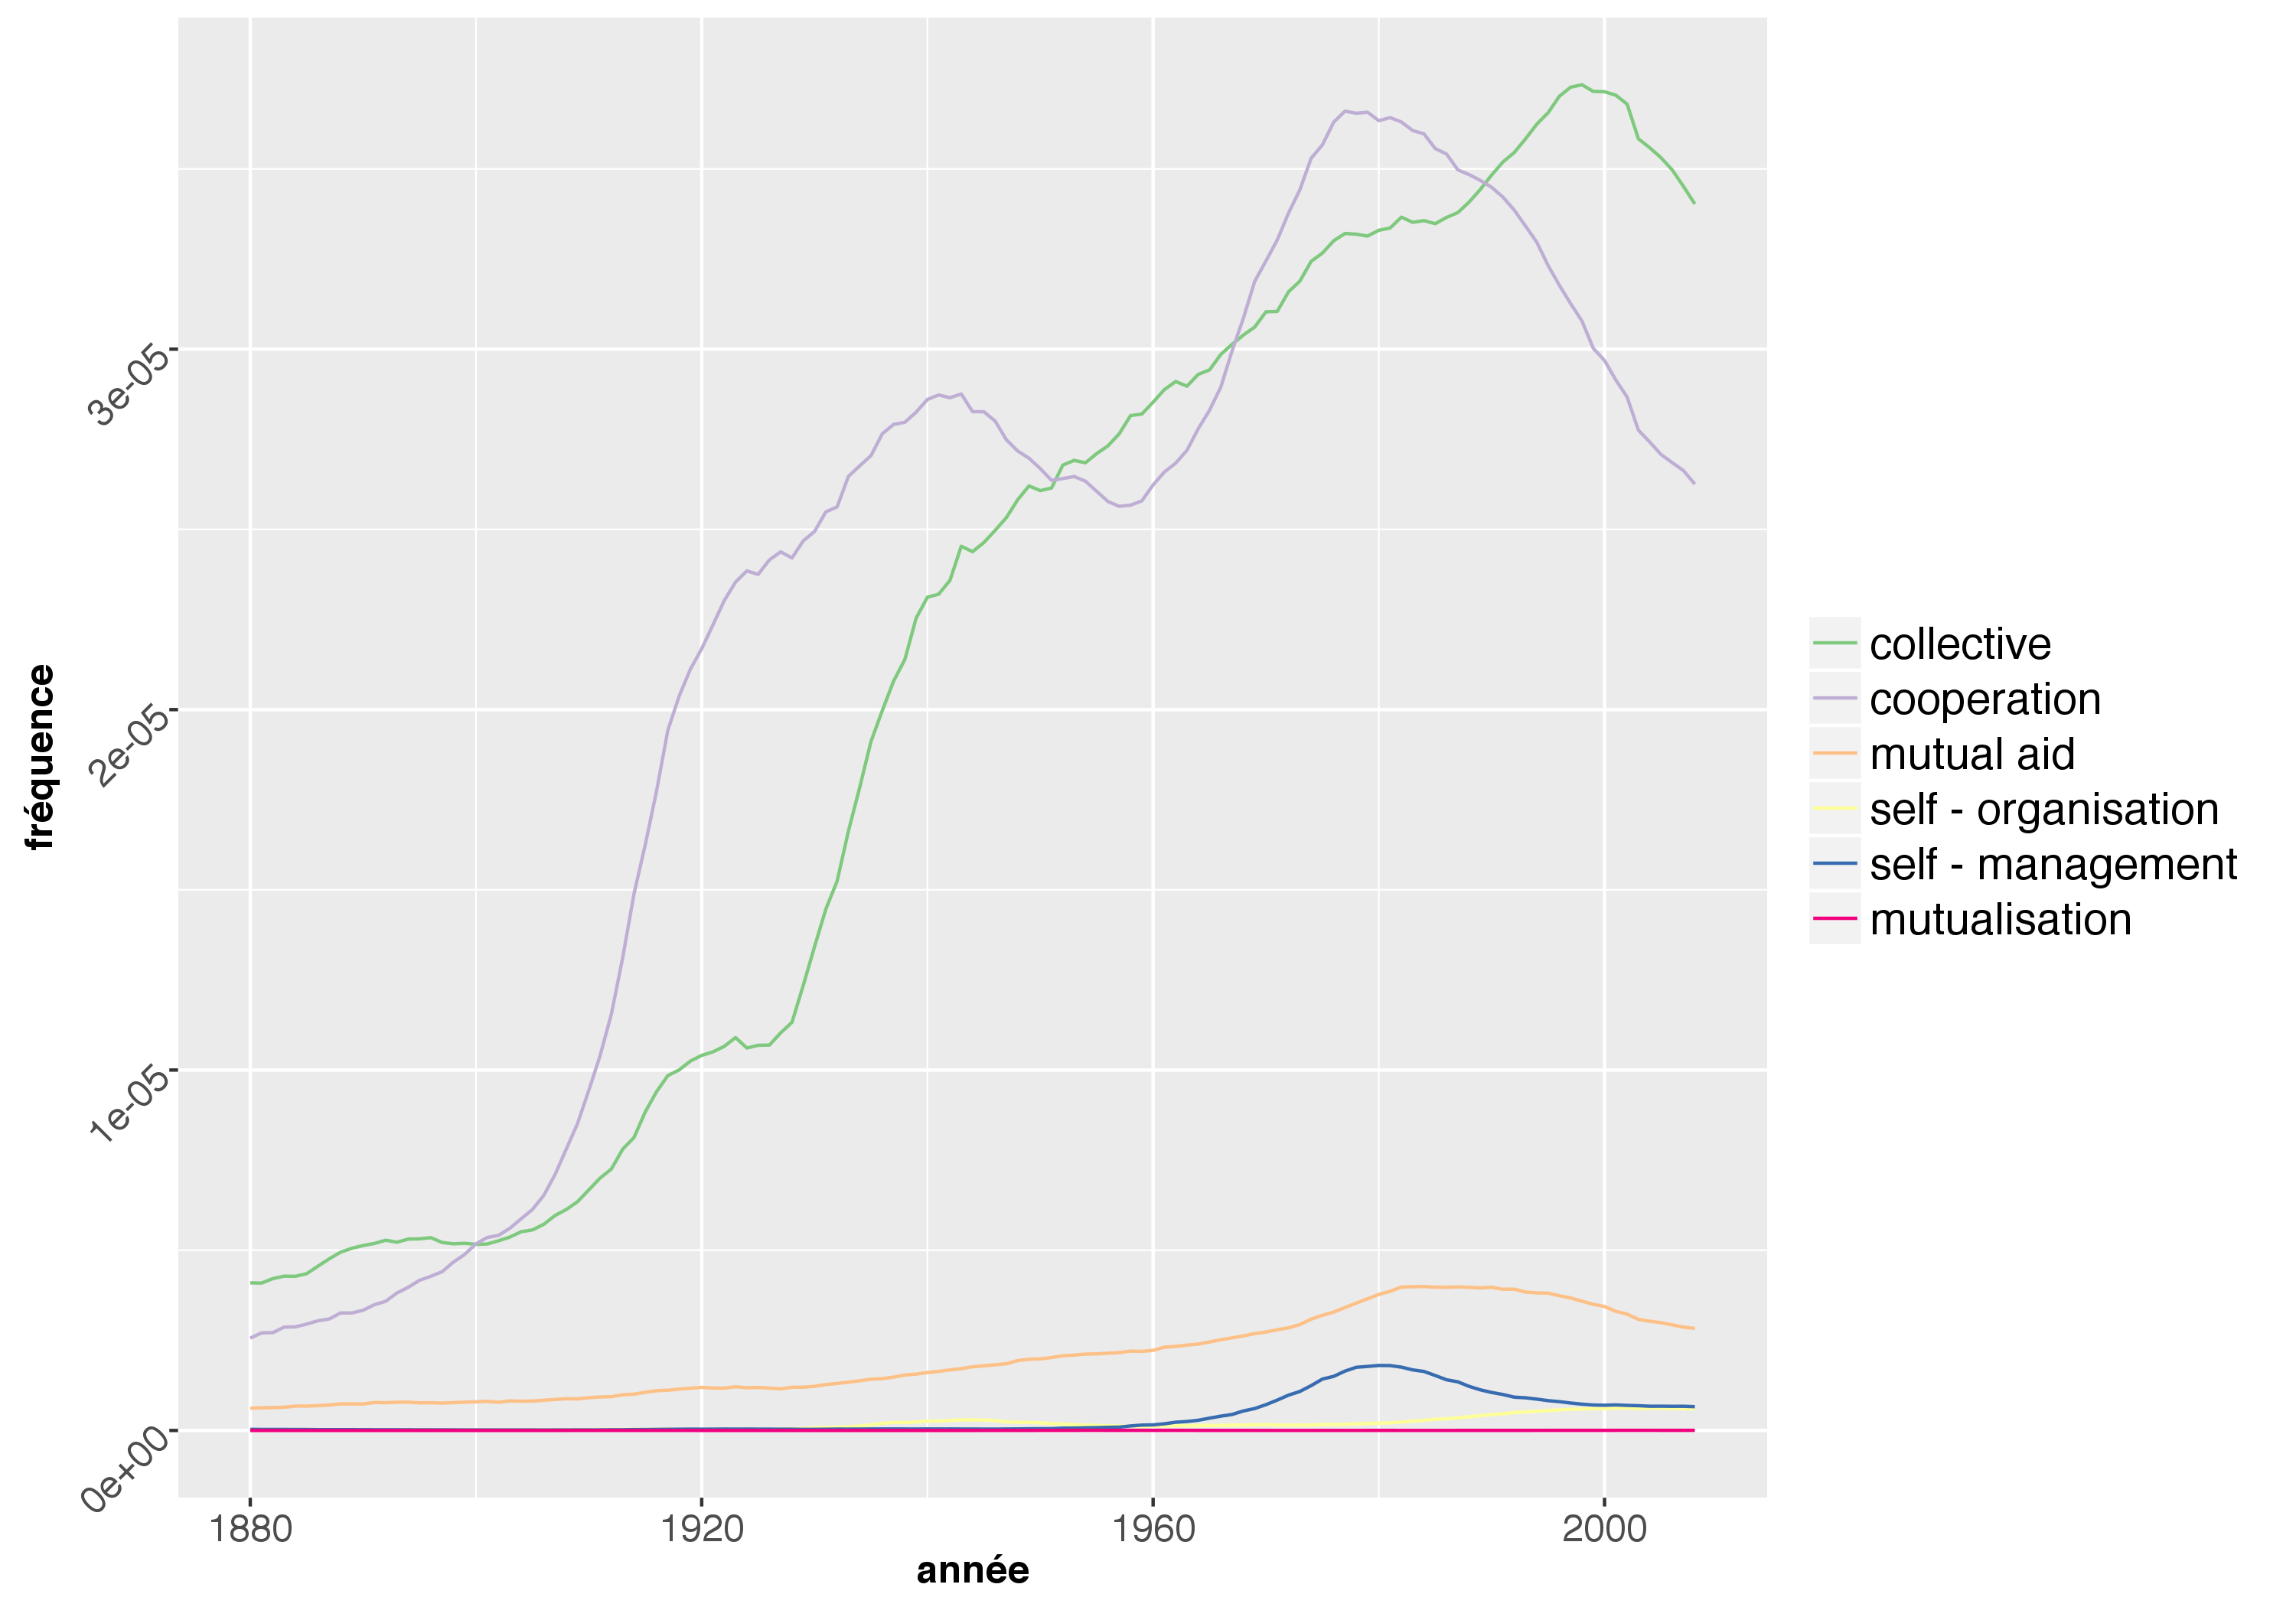
\includegraphics[width = 1\textwidth]{img/ngram_self}
\end{figure}
\small{source : google Ngram}

\end{frame}

%-=-=-=-=-=-=-=-=-=-=-=-=-=-=-=-=-=-=-=-=-=-=-=-=
%	FRAME:
%-=-=-=-=-=-=-=-=-=-=-=-=-=-=-=-=-=-=-=-=-=-=-=-=

\begin{frame}[c]{Usage des mots : français}
\vspace{-2em}
\begin{figure}
	\centering
	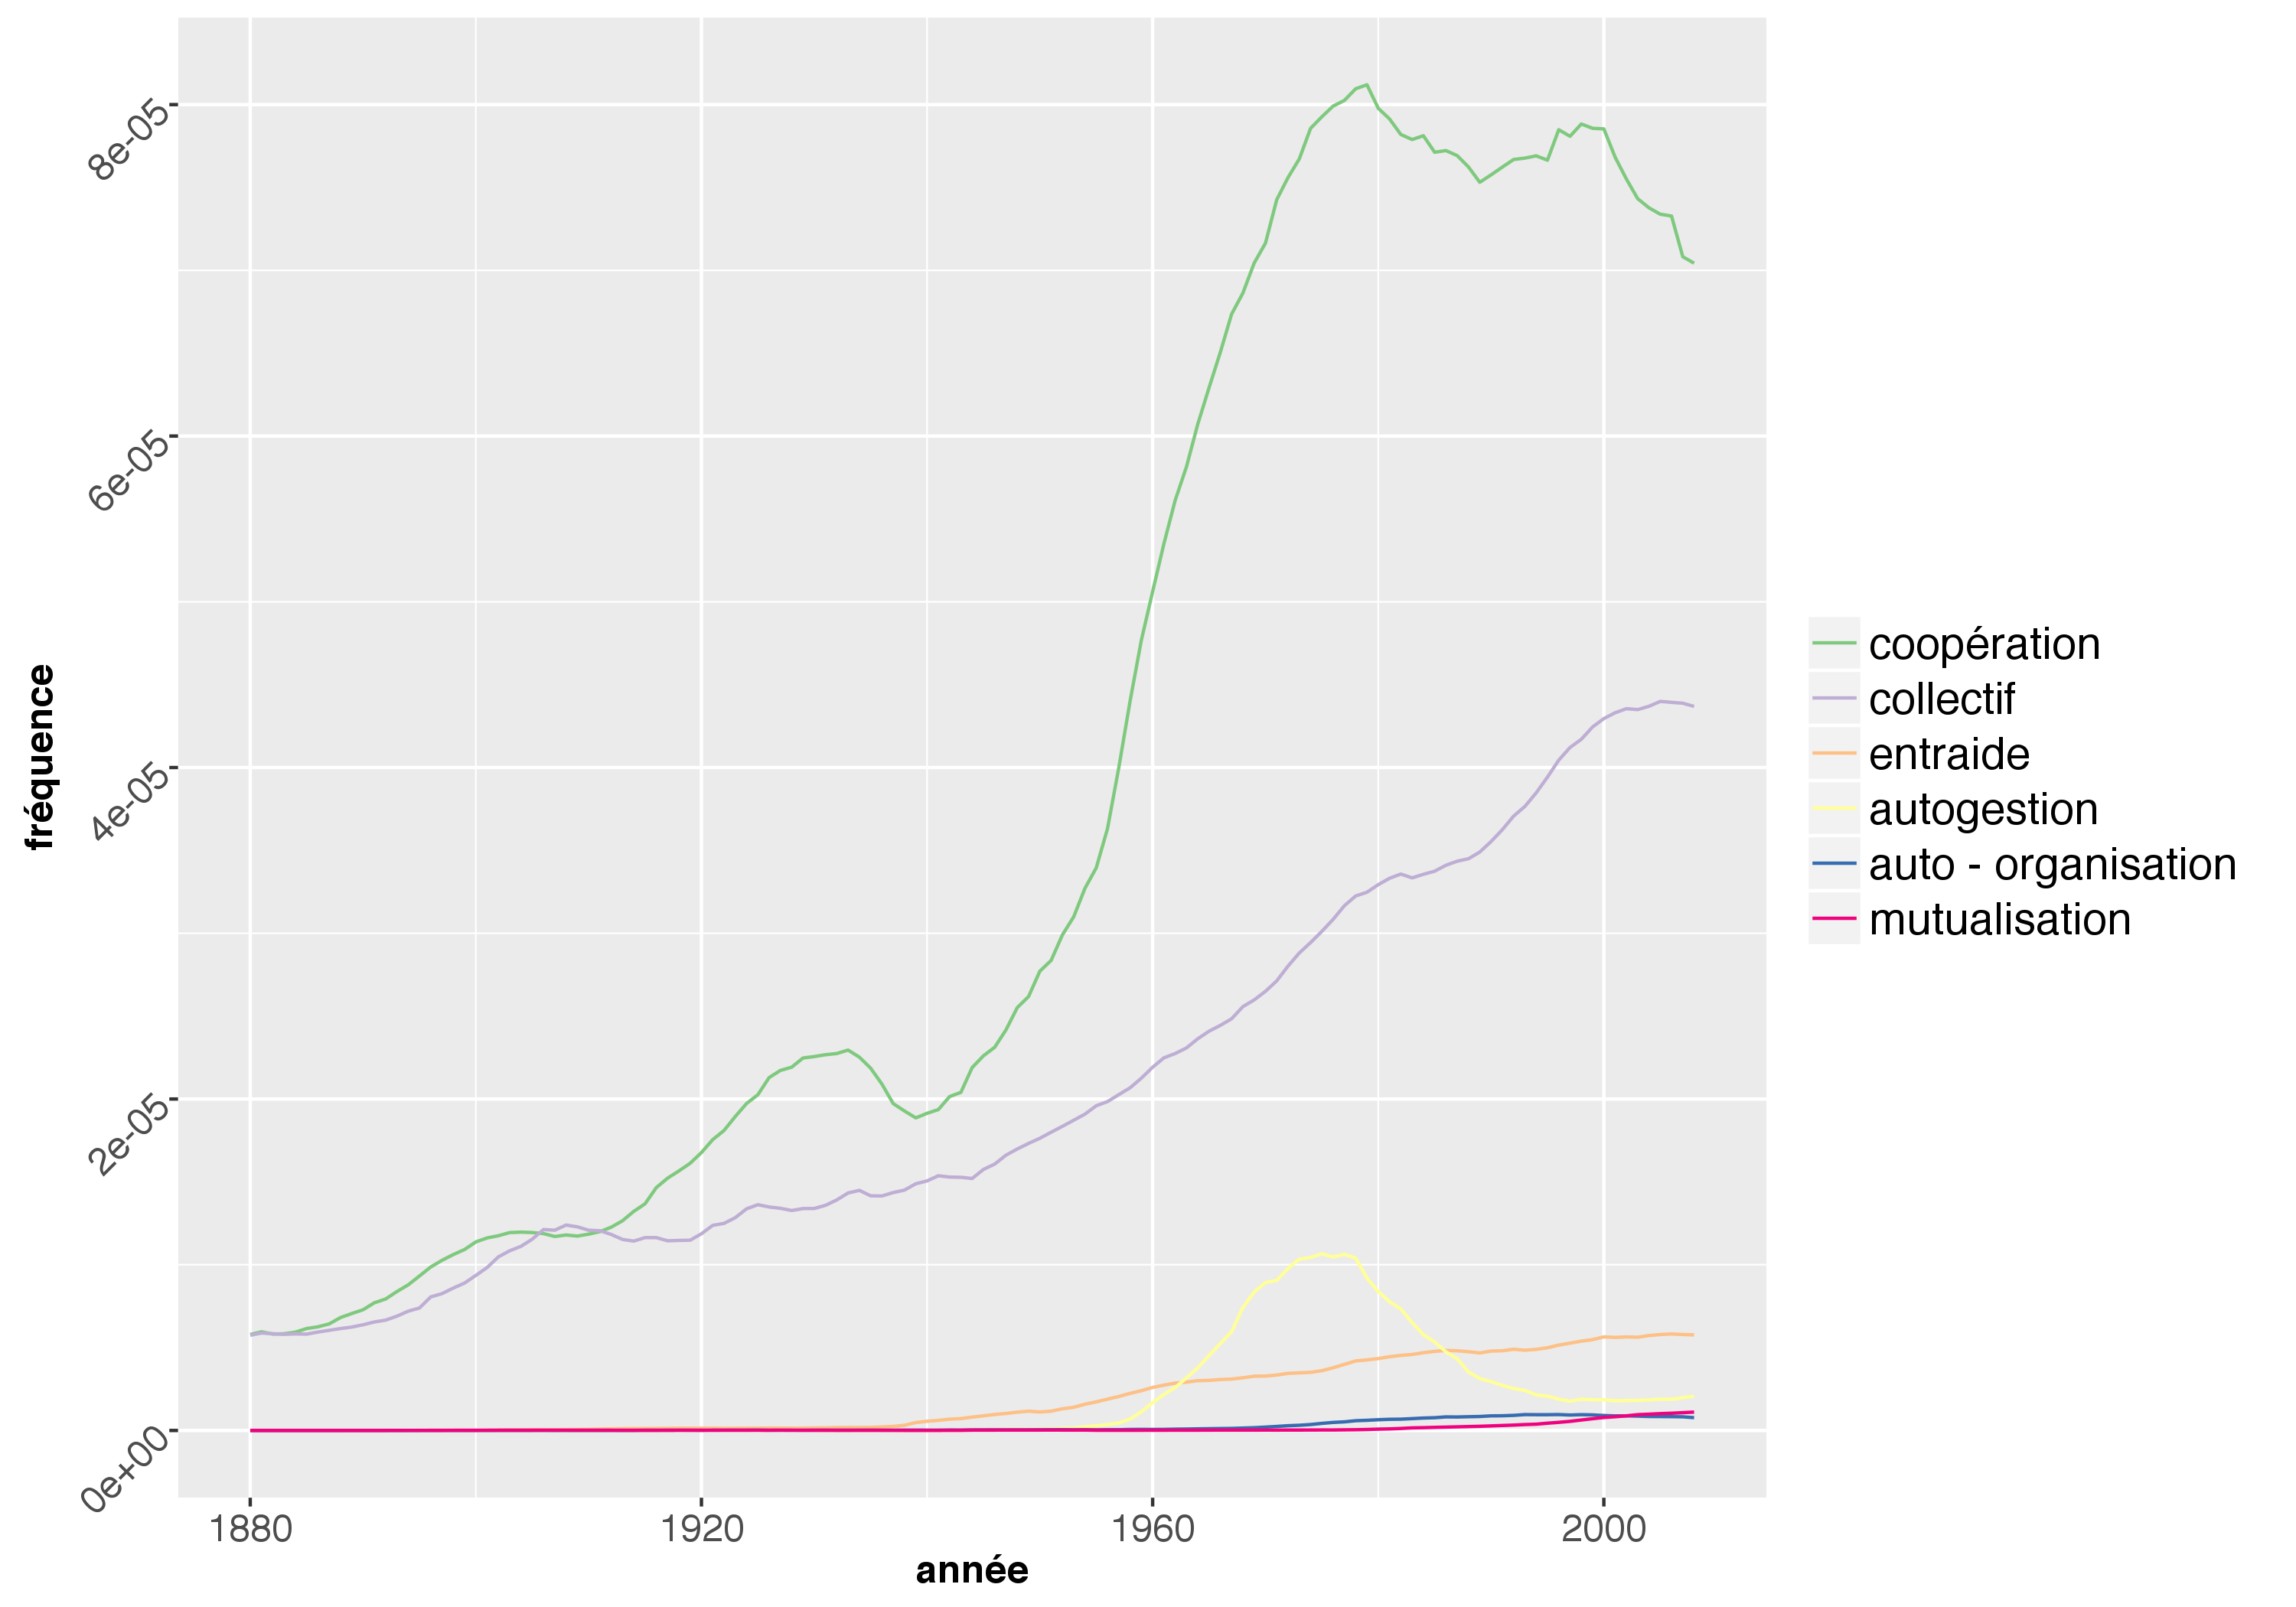
\includegraphics[width = 1\textwidth]{img/ngram_auto}
\end{figure}
\small{source : google Ngram}

\end{frame}

%-=-=-=-=-=-=-=-=-=-=-=-=-=-=-=-=-=-=-=-=-=-=-=-=
%	FRAME:
%-=-=-=-=-=-=-=-=-=-=-=-=-=-=-=-=-=-=-=-=-=-=-=-=

\section{Contexte geographique}
%-=-=-=-=-=-=-=-=-=-=-=-=-=-=-=-=-=-=-=-=-=-=-=-=
%	FRAME:
%-=-=-=-=-=-=-=-=-=-=-=-=-=-=-=-=-=-=-=-=-=-=-=-=

\begin{frame}[c]{La SAU irriguée en France}
\vspace{-2em}
\begin{figure}
	\centering
	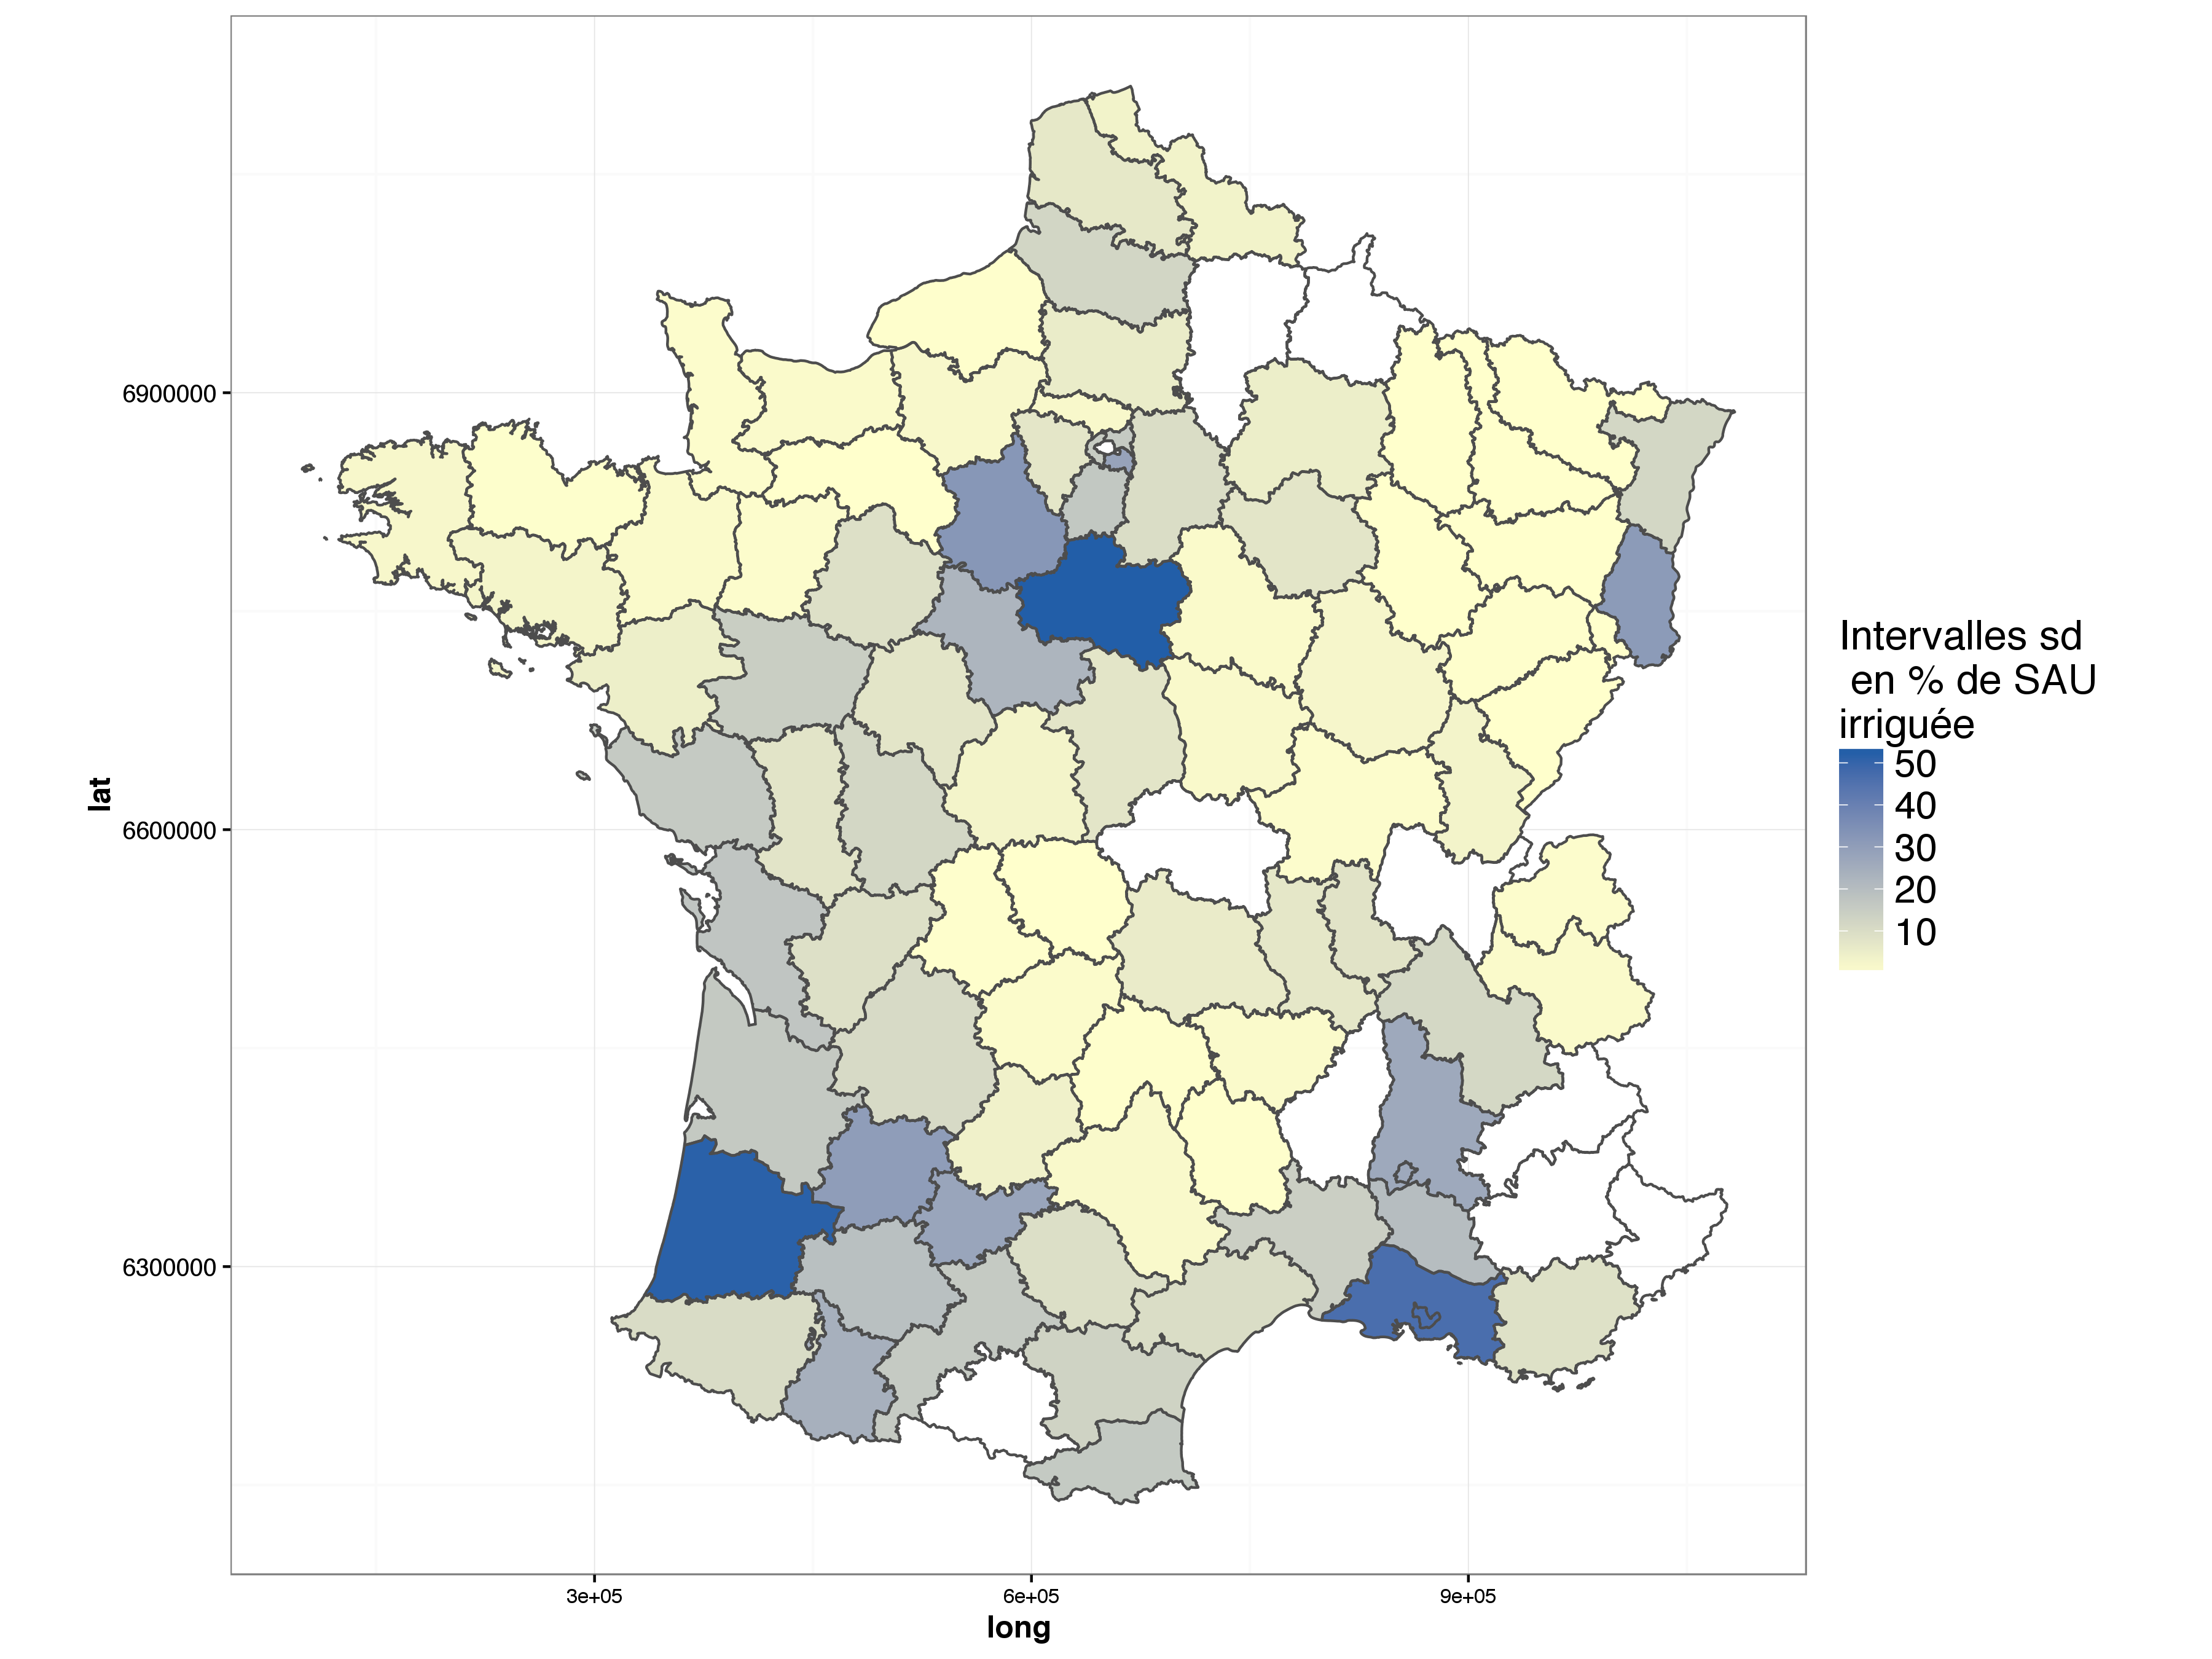
\includegraphics[width = 0.8\textwidth]{img/SAU}
\end{figure}
\small{Source : GEOFLA, Agreste -- Disar, RA 2010}

\end{frame}

%-=-=-=-=-=-=-=-=-=-=-=-=-=-=-=-=-=-=-=-=-=-=-=-=
%	FRAME:
%-=-=-=-=-=-=-=-=-=-=-=-=-=-=-=-=-=-=-=-=-=-=-=-=

\begin{frame}[c]{La place de l'irrigation collective}
\vspace{-2em}
\begin{figure}
	\centering
	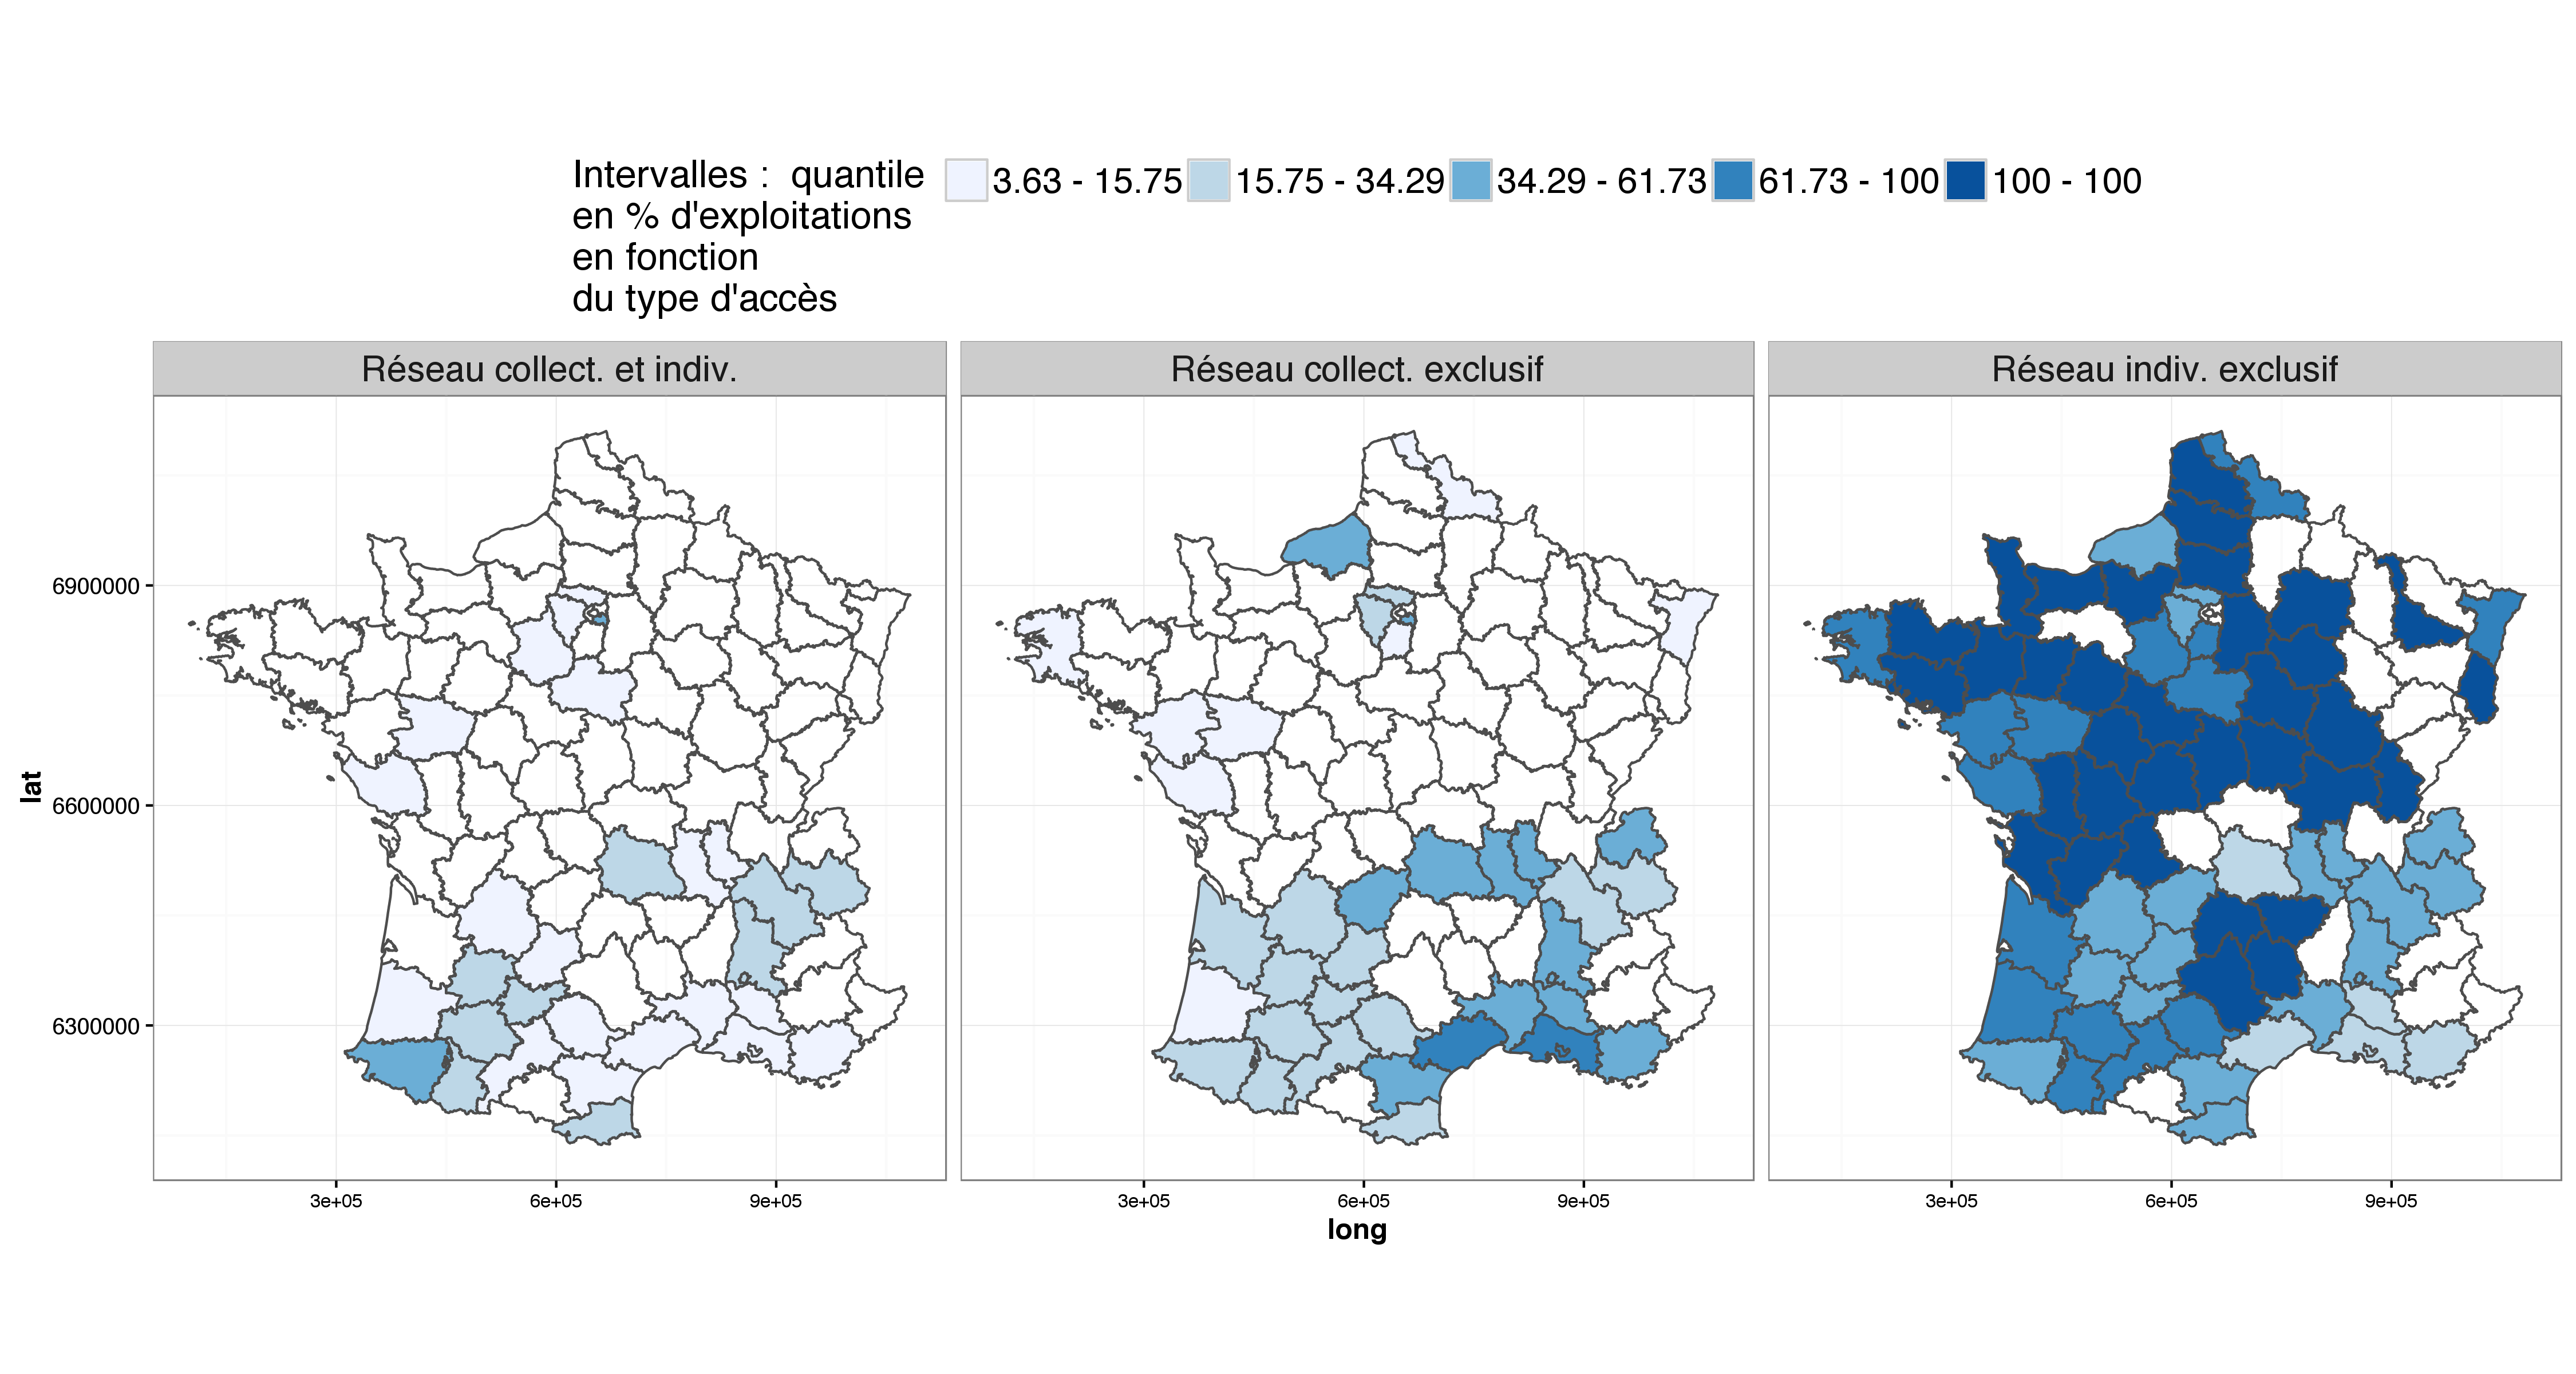
\includegraphics[width = 1\textwidth]{img/nb_irrigant2}
\end{figure}
\small{Source : GEOFLA, Agreste -- Disar, RA 2010}

\end{frame}

%-=-=-=-=-=-=-=-=-=-=-=-=-=-=-=-=-=-=-=-=-=-=-=-=
%	FRAME:
%-=-=-=-=-=-=-=-=-=-=-=-=-=-=-=-=-=-=-=-=-=-=-=-=

\begin{frame}[c]{Les ASAs en France}
\vspace{-3em}
\begin{figure}
	\centering
	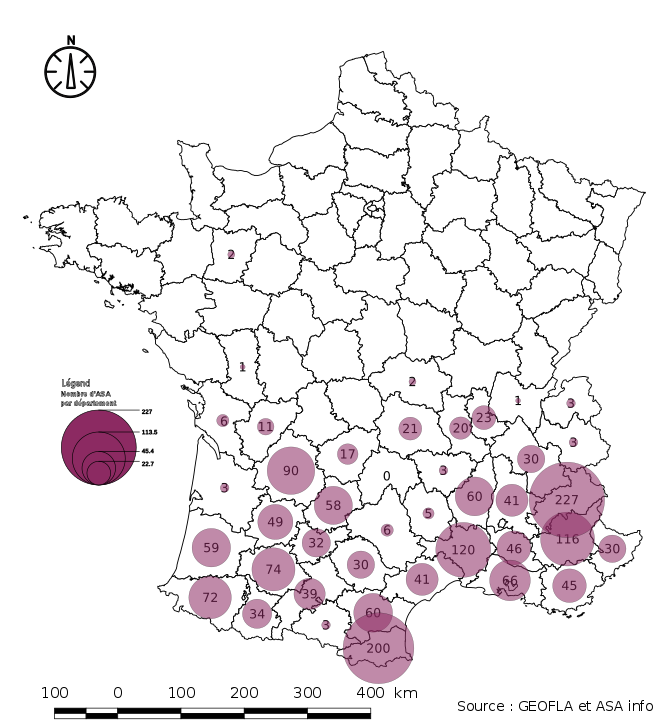
\includegraphics[width = 0.7\textwidth]{img/nbASA_dep}
\end{figure}


\end{frame}

%-=-=-=-=-=-=-=-=-=-=-=-=-=-=-=-=-=-=-=-=-=-=-=-=
%	FRAME:
%-=-=-=-=-=-=-=-=-=-=-=-=-=-=-=-=-=-=-=-=-=-=-=-=

\begin{frame}[c]{L'eau de surface dans les Pyrénées-Orientales}
\vspace{-4em}
\begin{figure}
	\hspace*{-0.6cm}
	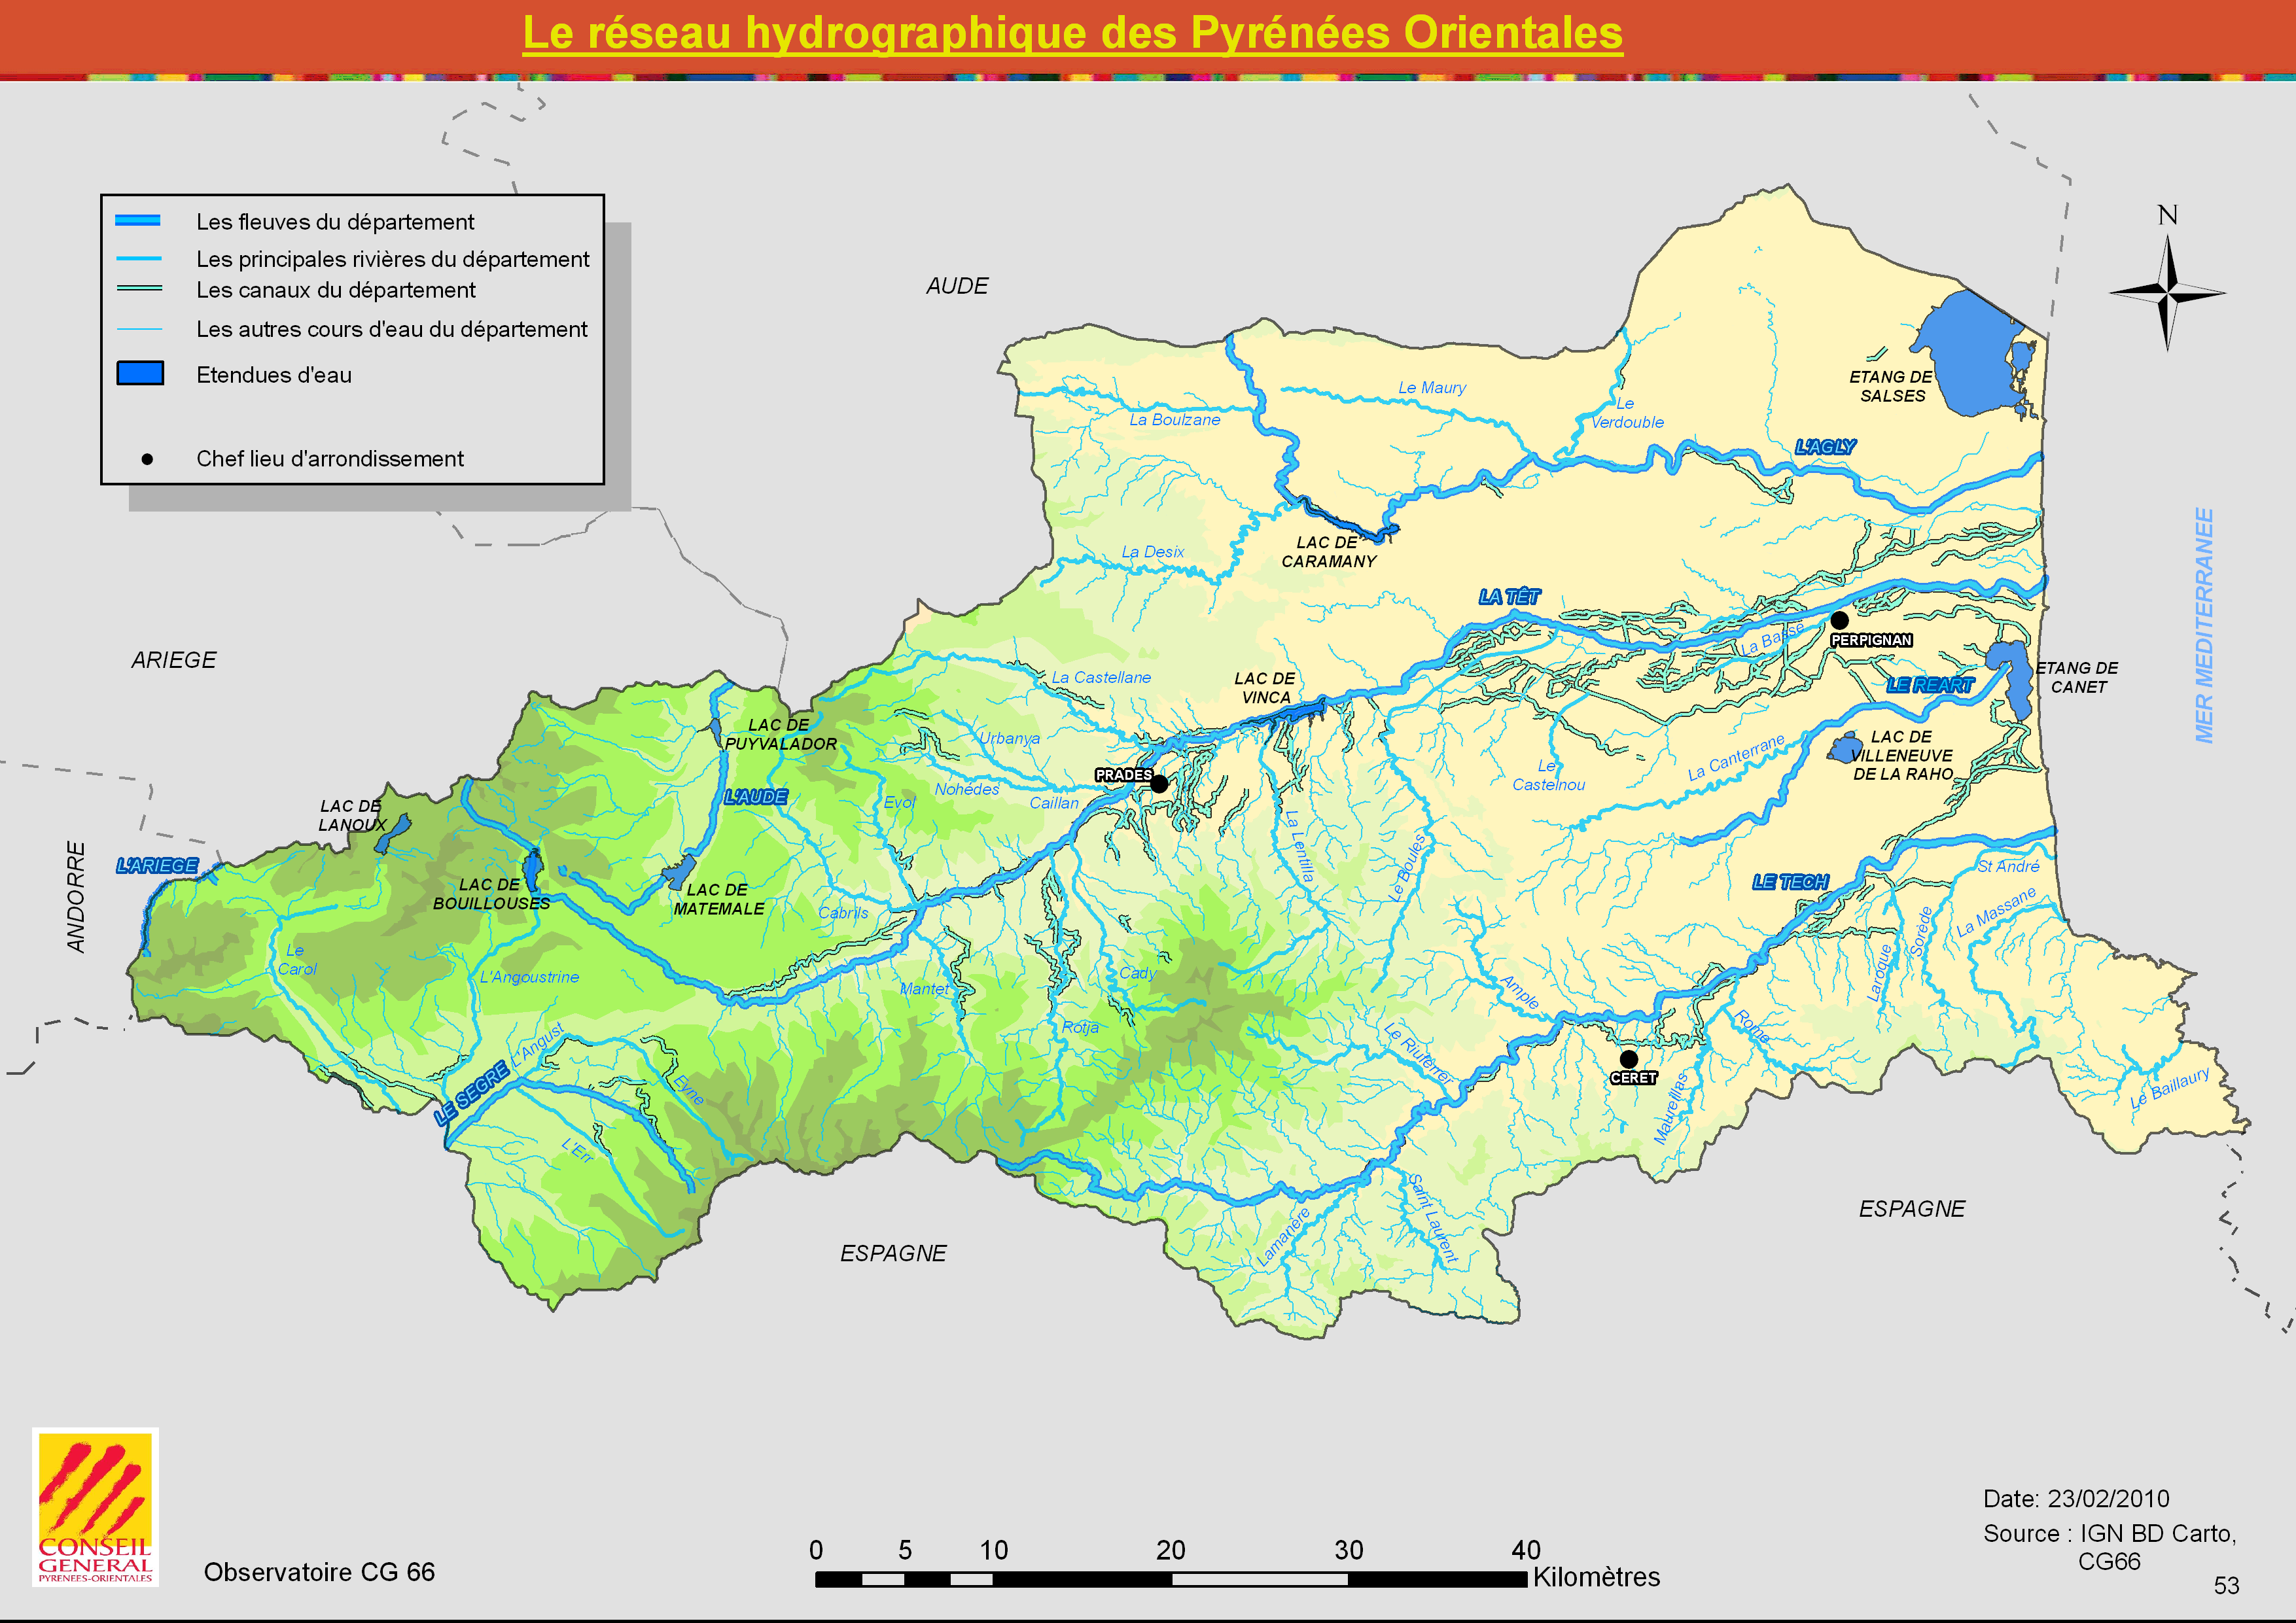
\includegraphics[width = 1.1\textwidth]{img/canaux_po}
\end{figure}


\end{frame}

%-=-=-=-=-=-=-=-=-=-=-=-=-=-=-=-=-=-=-=-=-=-=-=-=
%	FRAME:
%-=-=-=-=-=-=-=-=-=-=-=-=-=-=-=-=-=-=-=-=-=-=-=-=

\section{Focus sur une ASA : Corbere}

%-=-=-=-=-=-=-=-=-=-=-=-=-=-=-=-=-=-=-=-=-=-=-=-=
%	FRAME:
%-=-=-=-=-=-=-=-=-=-=-=-=-=-=-=-=-=-=-=-=-=-=-=-=

\begin{frame}[c]{Le barrage de Vinça }
\vspace{-0.5cm}

\startchronology[startyear=1900, stopyear=2000]
\chronoevent[markdepth=60pt]{1910}{Première étude}%order - furthest out first
\chronoevent{1920}{\cBlue{Crue}}
\chronoevent{1940}{\cBlue{Crue}}
\chronoperiode{1953}{1965}{$2^{nd}$ étude}
\chronoevent[markdepth=50pt, textwidth=2cm]{1954}{$1^{er}$ union des ASA}
\chronoevent[markdepth=20pt]{1976}{\cRed{Mise en eau}}
\chronoevent[markdepth=50pt, textwidth=3cm]{1989}{Station de pompage ASA de Corbère}
\stopchronology

\vspace{-1em}
Les objectifs du barrage :
\begin{itemize}
	\item réserve d'eau pour l'agriculture,
	\item ecrétage des crues,
	\item réserve d'eau potable.
\end{itemize}



\end{frame}

%-=-=-=-=-=-=-=-=-=-=-=-=-=-=-=-=-=-=-=-=-=-=-=-=
%	FRAME:
%-=-=-=-=-=-=-=-=-=-=-=-=-=-=-=-=-=-=-=-=-=-=-=-=

\begin{frame}[c]{Agriculture et irrigation dans les Pyrénées-Orientales}
\vspace{-3em}
\begin{figure}
	\hspace*{-1.1cm}
	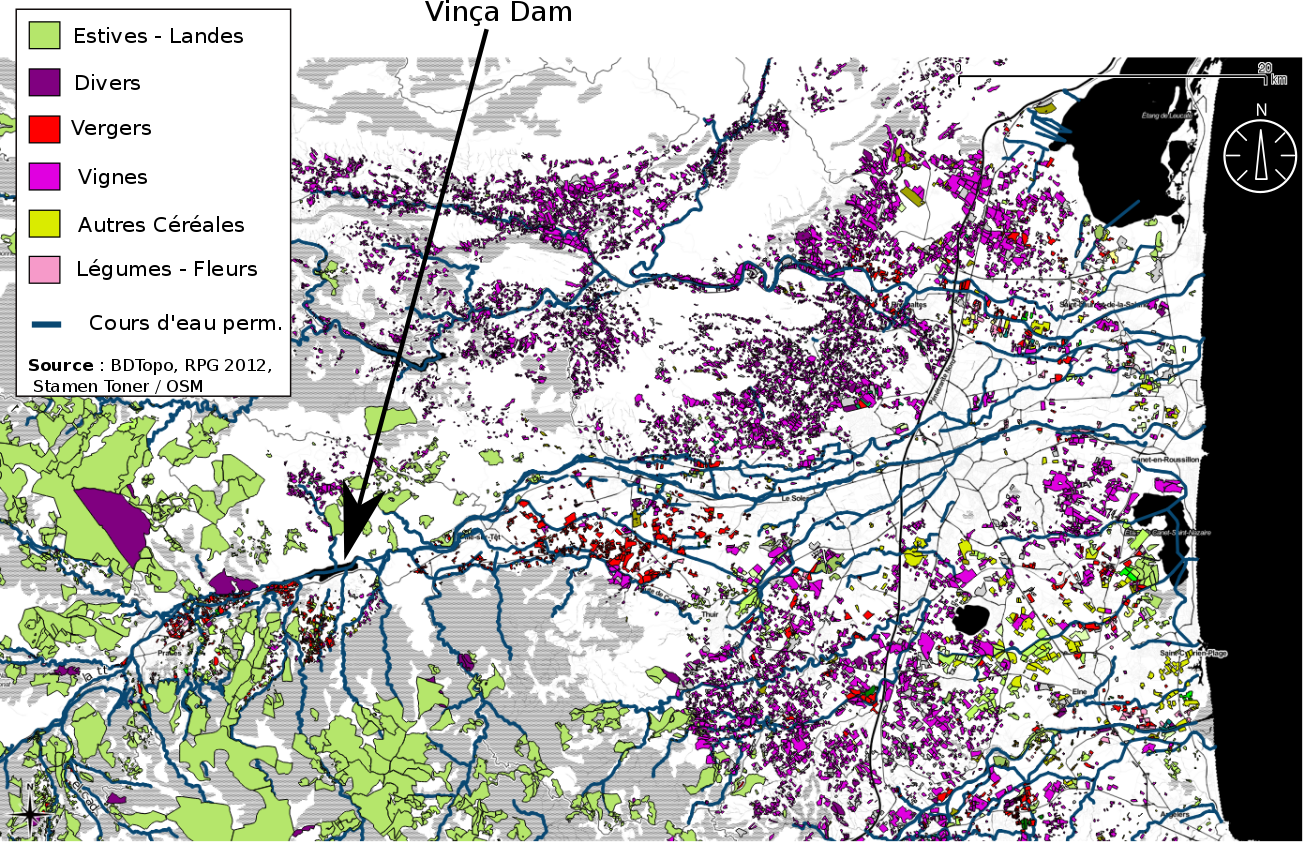
\includegraphics[width = 1.2\textwidth]{img/agriculture_aval_vinca}
\end{figure}


\end{frame}


%%-=-=-=-=-=-=-=-=-=-=-=-=-=-=-=-=-=-=-=-=-=-=-=-=
%%	FRAME:
%%-=-=-=-=-=-=-=-=-=-=-=-=-=-=-=-=-=-=-=-=-=-=-=-=
%
%\begin{frame}[c]{Parcours universitaire}
%
%
%
%
%\begin{alertblock}{These de doctorat : bourse regionale}
%\small{Sous la direction de É. \textbf{Rouvellac}, N. \textbf{Becu} et P. \textbf{Allée}. "Réflexions géographiques sur l’usage des systèmes multi-agents dans la compréhension des processus d’évolution des territoires viticoles de fortes pentes : le cas de la Côte Vermeille et du Val di Cembra"}.
%\end{alertblock}
%
%\end{frame}
%
%%-=-=-=-=-=-=-=-=-=-=-=-=-=-=-=-=-=-=-=-=-=-=-=-=
%%	FRAME: APERçU
%%-=-=-=-=-=-=-=-=-=-=-=-=-=-=-=-=-=-=-=-=-=-=-=-=
%
%\begin{frame}{Pratique et valorisation de la recherche}
%\vspace{-2em}
%\begin{itemize}
%	\item Une activité de recherche à l'international : France, Italie, Maroc,
%	\item Implication dans de nombreux travaux collectifs~: 6 projets de recherche (COMMONS, LittoSim, LACCAVE, ANR TerViClim, VitiTerroir, etc.),
%	\item Travaux interdisciplinaires avec : des économistes, des écologues, des agronomes, des écophysiologues, des climatologues, etc.
%\end{itemize}
%Publication ces 5 dernières années (doctorat + post-doctorat): 
%\small{
%\begin{itemize}
%	%\begin{itemize}
%		\item \textbf{Revues à comité de lecture} : 10
%		\item \textbf{Communications}  :  9 + 2
%		\item \textbf{Chapitres d'ouvrage} : 2
%		\item \textbf{Thèse de doctorat} : 1
%	%\end{itemize}
%\end{itemize}
%}
%\end{frame}
%
%
%%-=-=-=-=-=-=-=-=-=-=-=-=-=-=-=-=-=-=-=-=-=-=-=-=
%%
%%	SECTION: CONCLUSION
%%
%%-=-=-=-=-=-=-=-=-=-=-=-=-=-=-=-=-=-=-=-=-=-=-=-=
%\section*{Conclusion}
%
%%-=-=-=-=-=-=-=-=-=-=-=-=-=-=-=-=-=-=-=-=-=-=-=-=
%%	FRAME:
%%-=-=-=-=-=-=-=-=-=-=-=-=-=-=-=-=-=-=-=-=-=-=-=-=
%
%\begin{frame}[c]{Conclusion}
%\vspace{-2em}
%\begin{block}{\textsc{Atouts :}}
%	\begin{itemize}
%		\item Géographe et modélisateur → interface facilitée entre les disciplines
%		\item Un réseau de collaborations interdisciplinaires et inter-instituts (INRA, CIRAD, CNRS)
%		\item Un réseau international (Italie, Maroc, France)
%	\end{itemize}
%\end{block}
%\begin{exampleblock}{Competences}
%	\begin{itemize}
%		\item Maîtrise de différentes plateformes SMA, analyse de sensibilité, couplage de modèles, statistiques, géomatique %\includegraphics[width=0.8cm]{img/Logo_OSGeo}
%		\item Entretien, animation de sessions de jeux sérieux
%	\end{itemize}
%\end{exampleblock}
%
%\end{frame}

%-=-=-=-=-=-=-=-=-=-=-=-=-=-=-=-=-=-=-=-=-=-=-=-=
%	FRAME: MERCI DE VOTRE ATTENTION
%-=-=-=-=-=-=-=-=-=-=-=-=-=-=-=-=-=-=-=-=-=-=-=-=
{
\usebackgroundtemplate{
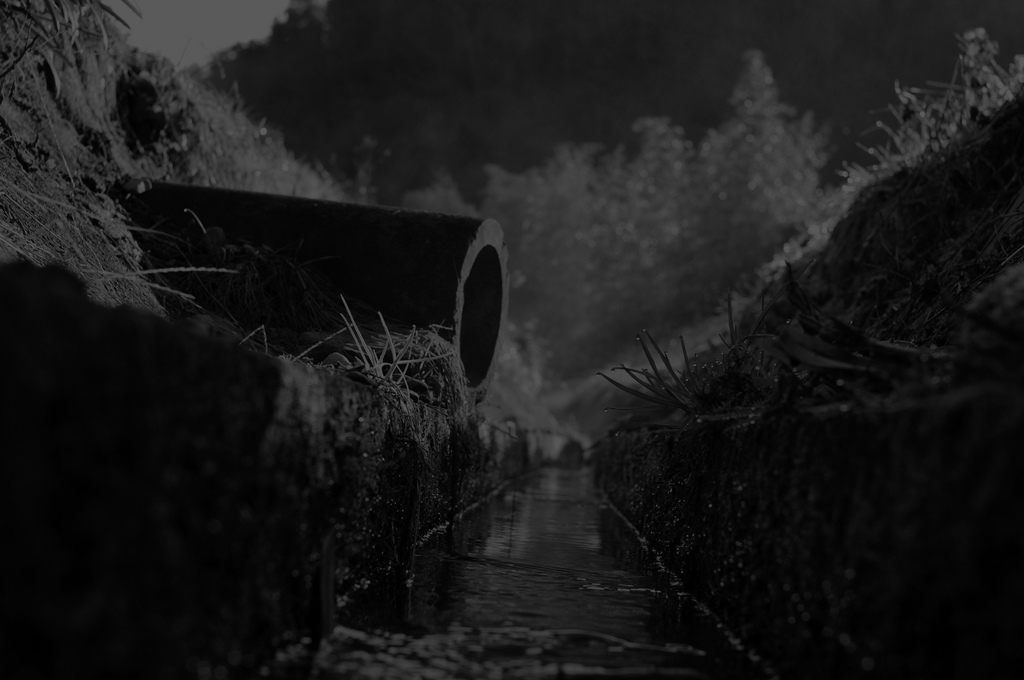
\includegraphics[width=\paperwidth]{img/fin.jpg}}%
\begin{frame}
  \vspace{-1em}  
  \begin{minipage}[t][.8\textheight]{\textwidth}
    \color{\cnGrey}{\LARGE{Merci de votre attention}}

    \vfill

  \hfill \small{Crédit photo : Thomas m-louis. sur 
\includegraphics[height=0.55cm]{img/flickr_logo}}
  \end{minipage}
  \vspace{-3em}
  \centering
	Vous pouvez retrouver cette présentation sur github
\includegraphics[height=0.85cm]{img/github}  
  
\end{frame}
}

\end{document}

%-====================================================
%  ANNEXES
%-====================================================

